\chapter{Értékelés}
\label{chap:ertekeles}
\section{Alternatíva - kódgenerálás}
A Gamma saját nyelvtanokkal rendelkezik, melyek Xtext segítségével vannak implementálva. Ez a technológia lehetővé teszi, hogy saját szintaxis alapján, lehessen kódot írni és EMF példánymodellt generálni a leírásból.

Ezt a mechanikát ki lehet használni a modell transzformáció alternatívájaként: a MagicDraw modellből Gamma Statechart Language szintaxisának megfelelő kódot lehetne generálni és ezt Xtext segítségével leparse-olni.

A visszakövethetőség is megoldható, ehhez a nyelvtant annotációkkal kéne kibővíteni, amik jelölnék az eredeti elemeket.

Ennek előnye, hogy a kimeneteket utána tovább lehetne importálni Eclipse-be és abban folytatni a fejlesztést.

Hátránya viszont, hogy a skálázhatóságot sokkal nehezebb megoldani, és kevésbé flexibilis mint a transzformáció.

\section{Plug-in teljesítménye}

A plug-in teljesítményét leginkább az jellemzi, hogy mennyi idő alatt képes végrehajtani a MagicDraw - Gamma transzformációt. Ennek meghatározására szolgálnak az alábbi mérések. Ezek célja a modell elemek számának és a végrehajtáshoz szükséges idő kapcsolatának vizsgálata.

\subsection{Mérések elvégzéséhez használt specifikációk}

\begin{table}[!h]
	\footnotesize
	\centering
	\begin{tabular}{ l r }
		Processzor & Intel i7-4770 @ 3.40GHz 3,40GHz \\
		Ram memóra & 8Gb\\
		Operációs rendszer & Windows 10 Pro \\
		Java verzió & Java 8 (181) \\
		MagicDraw verzió & 18.5 \\
		MagicDraw maximális heap méret & 2433Mb
	\end{tabular}
	\caption{Méréshez használ specifikációk}
	\label{table:gepspec}
\end{table}

\subsection{Egyszerű állapotgépek triggerrel}

Az egyszerű állapotgépek nem tartalmaznak csak állapotokat állapotátmeneteket és \emph{Signal Event Trigger}eket. A mérések hat különböző mintán lettek futtatva ezeket \aref{table:meres1}. táblázat szemléltei.

\begin{table}[H]
	\footnotesize
	\centering
	\begin{tabular}{ l r r r r r r}
		Név: & m1 & m2 & m3 & m4 & m5 & m6 \\ \hline
		Állapotok száma:  & 10 & 50 & 100 & 500 & 1000 & 2000 \\
		Állapotátmenetek száma: & 10 & 46 & 91 & 461 & 821 & 1641 \\
		\emph{Signal Event Triggerek} száma: & 9 & 45 & 90 & 460 & 820 & 1640
	\end{tabular}
	\caption{Első méréshez használt modellek}
	\label{table:meres1}
\end{table}

A mérések egymás után lettek futtatva ugyan azon a modellen új elemek felvételével az eredményeket \aref{fig:meres1}. ábra szemlélteti. Minden elemet ugyan az a régió tartalmazott és csak egy állapottérkép volt a modellben. Az állapotok és állapotátmenetek tíz hosszú láncokat alkottak. Minden leképzés után a leképzett modell kiírásra került a háttértárra.

\begin{figure}[H]
	\centering
	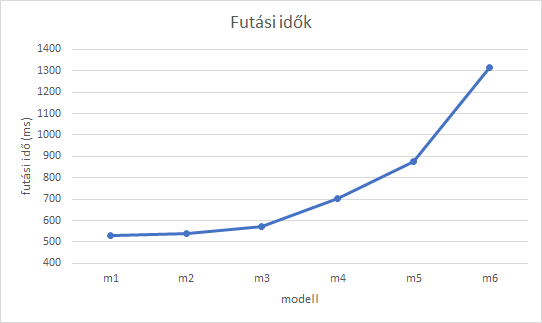
\includegraphics[keepaspectratio, width=140mm]{figures/meres1.png}
	\caption{Első mérés: transzformációk egymás után növekvő modellen}
	\label{fig:meres1}
\end{figure}

A grafikonról leolvasható, hogy az végrehajtási idő közel ugyan olyan arányban nőtt mint ahogy a modell mérete növekedett.

\subsection{Egyszerű állapotgépek őrfeltétellel}

A következő mérések során az állapotátmenetekre őrfeltételek kerülnek. Ezek leképzése Xtext parsert használ. Ennek a méréseknek a célja megvizsgálni az \emph{parse}-olás okozta teljesítmény romlást. Az új modellek és elemszámaikat \aref{table:meres2}. táblázat tartalmazza, az őrfeltétel a következő kifejezés:
\begin{lstlisting}
	true = (true and true) or a > 12
\end{lstlisting}

\paragraph{Megjegyzés:} az őrfeltételben használt \verb+a+ változó deklarálva lett az állapotgépen ennek a leképzése is megvalósul, azonban feltételezhető, hogy ez nem befolyásolja érdemben a mérést.

\begin{table}[H]
	\footnotesize
	\centering
	\begin{tabular}{ l r r r r r r}
		Név: & m1 & m2 & m3 & m4 & m5 & m6 \\ \hline
		Állapotok száma:  & 10 & 50 & 100 & 500 & 1000 & 2000 \\
		Állapotátmenetek száma: & 10 & 46 & 91 & 461 & 821 & 1641 \\
		\emph{Signal Event Triggerek} száma: & 9 & 45 & 90 & 460 & 820 & 1640 \\
		Őrfeltételek száma: & 9 & 45 & 90 & 460 & 820 & 1640
	\end{tabular}
	\caption{Második méréshez használt modellek}
	\label{table:meres2}
\end{table}

\begin{figure}[H]
	\centering
	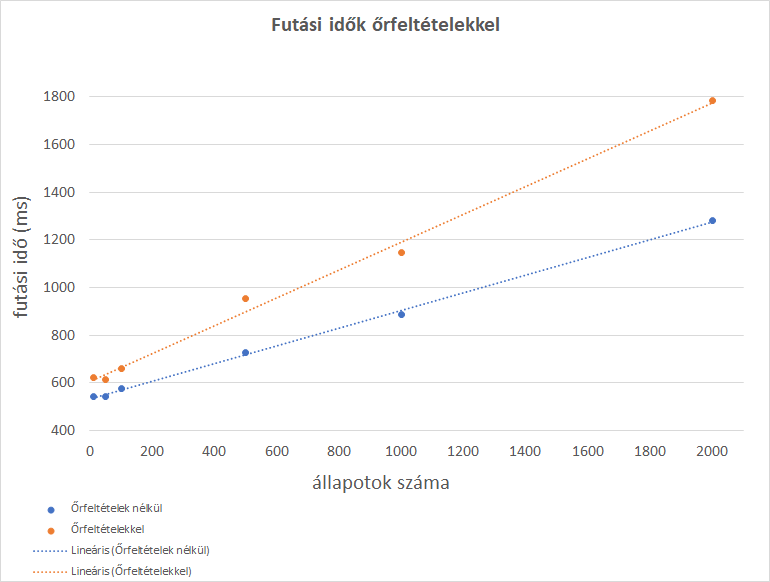
\includegraphics[keepaspectratio, width=140mm]{figures/meres2.png}
	\caption{Második mérés: futási idők őrfeltételekkel}
	\label{fig:meres2}
\end{figure}

Az őrfeltételek alkalmazása minden állapotátmeneten jelentősen megnövelte a futási időt átlag 20-25\%-al, ennek különösen a nagy modellek esetében lehet jelentősége.












